\documentclass[../main.tex]{subfiles}
\begin{document}
Java è un linguaggio di programmazione fortemente tipicizzato, ogni variabile e ogni espressione ha un tipo conosciuto al momento 
della compilazione. Ecco uno schema con i principali tipi di dato:
\begin{figure}[h]
    \centering
    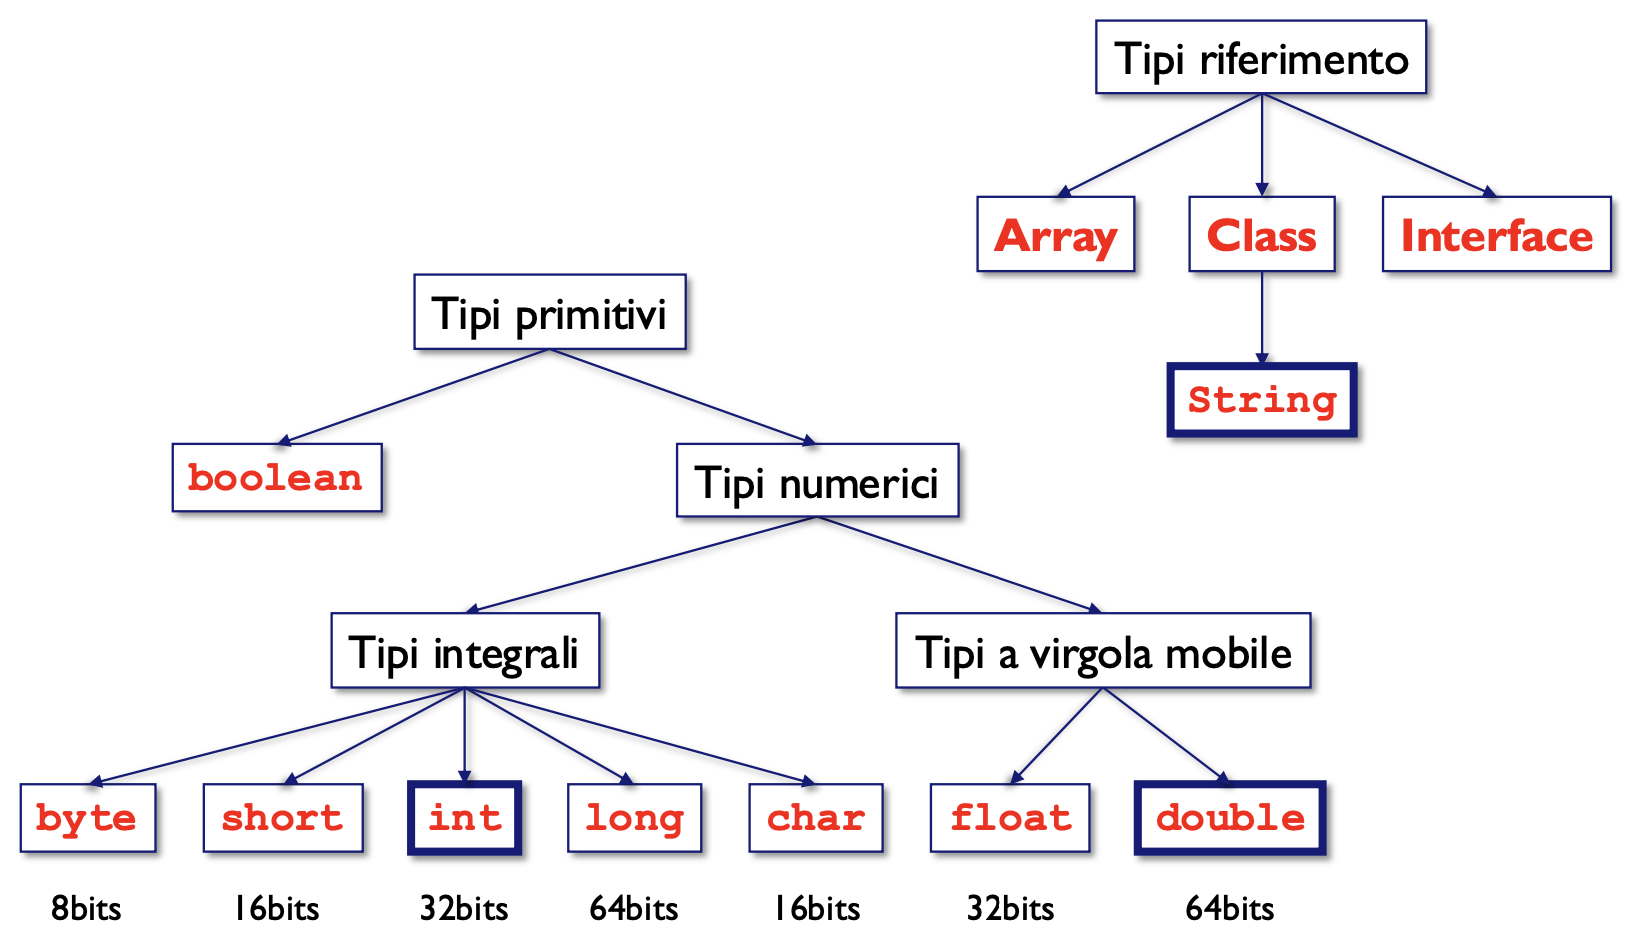
\includegraphics[width=1\textwidth]{../images/tipiDato.png}
\end{figure}

\subsection{boolean}
Il tipo \code{boolean} può assumere esclusivamente due valori: \code{true} e \code{false}. I valori booleani si ottengono anche dalla
valutazione di espressioni condizionali, ad esempio:
\begin{lstlisting}[style=java]
    boolean risultato = tasso > 0.05;
\end{lstlisting}

\subsection{Tipi numerici}
\subsubsection{Interi}
I tipi numerici interi sono rispettivamente \code{byte}, \code{short}, \code{int} e \code{long}. L'unica differenza tra di essi
è il range di numeri che è possibile rappresentare. Per valori ancora più grandi è possibile utilizzare il tipo di dato
\code{java.math.BigInteger}.

\subsubsection{char}
Serve per rappresentare i singoli caratteri. Esso permette l'utilizzo dei caratteri \textbf{Unicode}, uno standard per la rappresentazione
consistente del testo. Ad ogni carattere è assegnato un valore numerico ed è quindi possibile fare operazioni aritmetiche sui caratteri.

\subsubsection{Decimali}
È molto raro, ma ci sono alcuni numeri decimali che non possono essere rappresentati. In generale per comparare due valori decimali
non utilizziamo \code{==}:
\begin{lstlisting}[style=java]
    static final double EPSILON = 1e-8; //1 * 10^-8
    if(Math.abs(a-b) < EPSILON) { //confronta a e b
        ...
    }
\end{lstlisting}
I tipi decimali utilizzati solitamente sono \code{float} e \code{double}, per valori ancora più grandi è possibile utilizzare il tipo
di dato \code{java.math.BigDecimal}.



\end{document}